
\chapter{General discussion and research outlook}
\label{chap9}
\minitoc

Intrusive  magmatism  plays a  fundamental  role  in the  accretionary
processes of terrestrial crust.
 However, the processes by the magma is
intruded in  the crust  are still poorly  understood.  While  field or
remote  observations  can  sometimes  provide the  dimension  and  the
morphology of these  magmatic intrusions, they often  does not provide
information the intrusion process itself.



\section{Toward a general model for shallow magmatic intrusion}
\label{sec:toward-general-model}

\subsection{Summary}
\label{sec:summary}

\citet{Michaut:2011kg} originally  provides an  elastic-plated gravity
current  model  which  directly  links  the  observed  deformation  to
physical parameters of the  intrusion. In particular, depending mainly
on the injection rate and the  intrusion depth, the model predicts two
regimes  of propagation  characterized  by  specific morphologies  and
scaling laws  for intrusion  thickness versus  length and  time.  This
model predicts the appropriate geometry  for both laccoliths and large
mafic sills.  However, we show  in Chapter \ref{chap2} that this model
underestimates the absolute dimension of these magmatic intrusions; in
particular, it  requires abnormally  high viscosity to  reconcile both
observations and predictions.

To get  some insights in the  effective flow viscosity, we  develop in
chapter \ref{C3-JFM}  and \ref{Heating} an  extension of the  model of
\citet{Michaut:2011kg} that  accounts for the cooling  of the current.
We show that  the coupling between the temperature field  and the flow
itself leads  to the formation of  a highly viscous region  at the tip
which slows  down the  spreading in both  regime.  The  intrusions are
predicted to be thicker and their dimension, especially in the bending
regime, are now consistent with the observation.

In Chapter  \ref{C5-chap6}, we  neglect the  cooling to  relax another
assumption of  the original model of  \citet{Michaut:2011kg}, i.e. the
constant thickness  of the  upper layer. In  particular, we  study the
effect of a  crater depression on top of the  intrusion.  We show that
the lithostatic barrier imposed by the crater wall at the periphery of
the depression prevents  the spreading of the  intrusion which instead
thickens.   This second  model  show predictions  consistent with  the
deformations observed at floor-fractured craters.

While  the crater  depression clearly  limits the  flow expansion  for
crater-centered intrusion,  one can  wonder about why  laccoliths stop
their propagation in the bending regime. Available data on terrestrial
laccoliths, used in combination with  the model, show that terrestrial
laccoliths probably do not stop  following the formation of the highly
viscous region at the intrusion front, as initially suggested. Instead
we propose that the decrease in  the injection rate is responsible for
their  solidification in  the bending  regime.  Nevertheless,  we also
show the  limit in  using field observation  to test  this hypothesis.
Numerous assumptions  on the  model parameters  are often  required to
compare observation and  model predictions which make  it difficult to
definitely conclude.

An  alternative  approach  to  validate  the  model  and  its  further
refinement could be  to use analogue experiments that  are designed to
produce  some feature  of the  natural system  at a  laboratory scale.
Indeed, in  such experiment, all the  parameters are known and  can be
controlled.  Furthermore, phenomenological  observations not predicted
by  the theory  could guide  further investigations  in the  intrinsic
mechanism that governs the dynamics.

\subsection{Second order modeling}
\label{sec:perspectives}

In Chapter  \ref{chap2}, \ref{C3-JFM} and \ref{Heating},  we show that
the local condition at the tip of the current controls the dynamics in
the  bending  regime.  For  a  sake  of  simplicity,  we used  a  thin
prewetting film  at the tip to  avoid the requirement of  any boundary
condition at  a genuine  front. Nevertheless,  a natural  extension of
this work  is the description  of a  proper boundary condition  at the
intrusion front.

\subsubsection*{Boundary condition}

A first step  would be to describe  the tip in term of  a fluid driven
fracture  instead of  the thin  prewetting  film. As  seen in  Section
\ref{C2-Toughness},  linear elastic  fracture mechanics  requires that
the  mode $I$  intensity  factor  $K_I$ equal  a  critical value,  the
fracture toughness  of the wall  rock $K_{c}$, for the  propagation to
occur.  This condition  is usually expressed in term  of an asymptotic
condition      on      the       crack      opening      at      $r=R$
\citep{Savitski:2002gy,Bunger:2005em,Bunger:2007vs,Detournay:2014fk}.

In  such  problem, the  lubrication  equation  is  thus coupled  to  a
description  of  the fracture  opening  based  on the  linear  elastic
fracture mechanics.  \citet{Bunger:2011cb} use  this approach to solve
the problem of  shallow magmatic intrusions and  found similar results
than  \citet{Michaut:2011kg}.  Interestingly,  they needed  values for
the fracture toughness $K_c$ two  or three orders of magnitudes larger
than  laboratory measurements  to agree  with the  observations, which
they attribute to  potentially crack blunting mechanism at  the tip of
laccoliths.  This  observation is consistent with  the rapid formation
of  a  highly viscous  plug  at  the  tip  of the  magmatic  intrusion
described in Chapter \ref{C3-JFM} and \ref{Heating}.

Nevertheless, this model also falls short to reproduce the geometry of
large  mafic sills.   In addition,  more realistic  model should  also
consider the process zone, i.e. the region of plastic rock deformation
near       the      leading       edge      of       the      fracture
\citep{Bunger:2008cl}. Furthermore,  the large negative  pressure that
developed at the front might cause desolved gasses to exsolve from the
magma.  With the formation and the  evolution of a gap filled with gas
at the  tip of the  current, the fluid and  the fracture front  do not
coincide with one  another, thus requiring the tracking  of two moving
boundaries.

Along      with      the     prewetting      film      regularization,
\citet{Anonymous:QWXp_4JV} propose  a second  regularization condition
where the tip of the elastic-gravity  current consists of a lag region
filled   with    gas   at    constant   negative    pressure   (Figure
\ref{C7-Sketch}).   They show  that the  solution depends  on the  gas
pressure  in the  tip  region  in similar  fashion  that the  solution
depends  on  the prewetting  film  thickness  in Chapter  \ref{chap2},
\ref{C3-JFM} and \ref{Heating}.
\begin{figure}[h!]
  \begin{center}
    \graphicspath{ {/Users/thorey/Documents/These/Manuscript/Figure/Chapter7/} }
    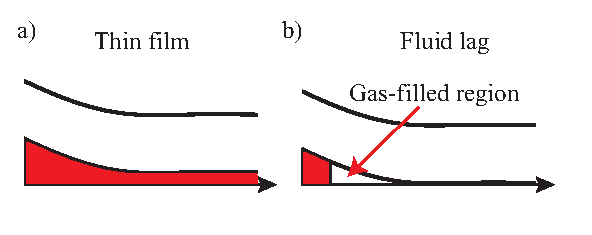
\includegraphics[scale=1.3]{Sketch.eps}
    \caption{Two different  regularization condition  at the  front of
      the current: a) thin prewetting film with thickness $h_f$ b) gas
      -filled region.}
    \label{C7-Sketch}
  \end{center}
\end{figure}
In particular, they show that
\begin{eqnarray}
  h_0&\propto& h_f^{-1/7}\nu^{-2/7}L^{10/7}~(\text{Thin film})\\
  h_0&\propto& \sigma^{1/9}\nu^{-2/9}L^{14/9}~(\text{Fluid lag})
\end{eqnarray}
where $L$  is the half  length of the  flow, $-\sigma$ is  the contant
negative  pressure  in  the  fluid   lag  and  we  have  rescaled  the
characteristic    thickness    and     time    by    $\nu^{1/4}$    in
\citet{Anonymous:QWXp_4JV}.    As   expected,    the   two   different
regularization conditions lead  to only minor change  in the thickness
to   length   relationship   ($10/7\sim  1.4$,   $14/9\sim   1.5   $).
Nevertheless, a  complete description of  the dynamics of  the cooling
gas-filled  region, where  the pressure  is not  a parameter  but self
consistently  determined,   would  surely  complete   the  description
provides in this thesis.

\subsubsection*{Stretching of the overlying layer}

If the thickness of the intrusion  $h_0$ becomes large compared to the
intrusion depth $d_c$, the  analysis described in Chapter \ref{C3-JFM}
and  \ref{Heating}  is  not  valid  anymore. It  could  be  the  case,
especially for felsic intrusions characterized by large injection rate
intruding a layer such that $d_c\lessapprox 500$ m. In such situation,
the stretching  of the  upper layer  can no  longer be  neglected when
calculating the elastic stresses and fluid pressure. The previous work
of \citet{Lister:2013ia} and \citet{Anonymous:QWXp_4JV} can be used to
extend the model in that direction.

\subsubsection*{Viscous heating instabilities}

Viscous heating  is another mechanism  not taken into account  in this
study  that would  participate  to the  dynamics  of shallow  magmatic
intrusions. Indeed, especially for large  values of $Pe$ where we have
shown  that the  temperature  gradient within  the  flow are  stronger
(Section  \ref{C4-sec:infl-therm-bound-el}),  the  effect  of  viscous
heating could  be important.  \citet{Costa:2005bq} have  already shown
that viscous heating plays an important role in the dynamics of fluids
with strongly temperature-dependent viscosity. In particular, for lava
tube, they show that the heat generated by viscous friction produces a
local  temperature increase  near  the tube  walls  with a  consequent
decrease  of   the  viscosity   which  may  dramatically   change  the
temperature             and              velocity             profiles
\citep{Costa:2002cj,Costa:2003wk,Costa:2005bq}.      The     important
gradients near  the tip  region or within  the thermal  boundary layer
could  present  favorable  conditions  for  the  development  of  such
instabilities.

\subsubsection*{Christmas tree structure}

In chapter \ref{Heating},  we show that a  significant thermal aureole
should develop in the wall rocks above the central flow region.  Apart
from  plastic rock  deformation  that might  develop  in the  encasing
rocks,  studying  the  possible  thermal  erosion  could  also  be  an
interesting thing to look at. For instance, above the feeder dyke, the
temperature are  expected to be  maximum which might  favor subsequent
dyke propagation.  This could potentially explain the nested structure
of   several   laccolith   complexes  reported   in   the   literature
\citep{E:2015tl,Rocchi:2010dn}.  Such dyke  formation would also limit
the size of the terrestrial laccoliths.

\subsection{Model validation}

In  this thesis,  we show  the limit  in using  field observations  to
validate the model. An alternative  approach to validate the model and
its further refinement  could be to use analogue  experiments that are
designed to produce some feature of the natural system at a laboratory
scale.  Indeed, in  such experiment, all the parameters  are known and
can  be controlled.   Furthermore,  phenomenological observations  not
predicted  by the  theory could  guide further  investigations in  the
intrinsic mechanism that governs the dynamics.

\section{Probing intrusive magmatism on terrestrial planets}
\label{sec:elast-plat-grav}

In this thesis, we show than theoretical mode, upon validation, can be
used to understand the intrusion process itself.


%%% Local Variables:
%%% mode: latex
%%% TeX-master: "../main"
%%% End:


%%% Local Variables:
%%% mode: latex
%%% TeX-master: "../main.tex"
%%% End:
